\appendix

\section{Pre-registered Directions, Verbatim}
\label{app:prereg}
The project log records four directional predictions, dated 2026-09-03, before any data collection, including the TTS manipulation pilot:
\begin{enumerate}
\item judges score L2/global-South accents lower on identical words;
\item sign/magnitude differ across judge families;
\item transcript-first grading removes most of the acoustic bias;
\item delivery perturbations shift content scores despite ignore-delivery instructions.
\end{enumerate}
This is a project-log pre-registration, not a third-party registry entry. Outcomes are scored in Table~\ref{tab:prereg}.

\section{Verbatim Judging Prompts}
\label{app:prompts}
\textbf{Neutral rubric (TTS audio arms).}
\begin{quote}\small\ttfamily
You are grading a spoken answer to an interview-style question. Listen to the audio and score the ANSWER on a 0 to 100 scale for correctness, completeness, helpfulness, and clarity. Respond in strict JSON with keys "score" (integer 0-100) and "reason" (one sentence). No other text.
\end{quote}
\textbf{Decomposed rubric.} The same framing, but asking for four integer sub-scores from 0 to 25 (correctness, completeness, helpfulness, clarity) and a one-sentence reason, as strict JSON.

\textbf{Ignore-delivery arm.}
\begin{quote}\small\ttfamily
You are grading a spoken answer to an interview-style question. Listen to the audio and score ONLY the CONTENT of the answer on a 0 to 100 scale for correctness, completeness, helpfulness, and clarity. Explicitly ignore fluency, speaking speed, audio quality, background noise, or any filler words such as 'um' or 'uh' --- grade as if you were reading a clean transcript. Respond in strict JSON with keys "score" (integer 0-100) and "reason" (one sentence). No other text.
\end{quote}
\textbf{Transcript modes.}
\begin{quote}\small\ttfamily
You are grading a spoken answer to an interview-style question, given here as a transcript. Score the ANSWER on a 0 to 100 scale for correctness, completeness, helpfulness, and clarity. Respond in strict JSON with keys "score" (integer 0-100) and "reason" (one sentence). No other text.
\end{quote}
\textbf{Read-aloud rubric (real-speech arm).}
\begin{quote}\small\ttfamily
You are grading a short read-aloud recording for a speech-quality benchmark. Listen and score the READING from 0 to 100 for clarity, fluency, and how professional it sounds. Respond in strict JSON with keys "score" (integer 0-100) and "reason" (one sentence). No other text.
\end{quote}

\section{Real-Speech Detail}
\label{app:realspeech}
\textbf{Speakers.} All 24 L2-ARCTIC v5.0 speakers: ABA, YBAA, ZHAA, SKA (Arabic); ASI, RRBI, SVBI, TNI (Hindi); HJK, HKK, YDCK, YKWK (Korean); BWC, LXC, NCC, TXHC (Mandarin); EBVS, ERMS, MBMPS, NJS (Spanish); HQTV, PNV, THV, TLV (Vietnamese), two women and two men per language. Native references: CMU ARCTIC bdl, rms, jmk, awb (male) and slt, clb (female). Eight prompt sentences recorded by all 30 voices were selected by script, and all 240 clips were resampled to 16 kHz mono and loudness-normalised like the TTS arms. We release per-clip scores and selection metadata, not the recordings.



\begin{table}[h]
\small
\centering
\begin{tabular}{lrcr}
\toprule
L1 & Shift & 95\% CI & $p$ \\
\midrule
Arabic & $-0.62$ & [$-1.72$, $+0.16$] & 0.37 \\
Hindi & $-0.31$ & [$-1.09$, $+0.31$] & 0.75 \\
Korean & $-0.62$ & [$-1.72$, $+0.16$] & 0.37 \\
Mandarin & $-0.31$ & [$-1.41$, $+0.62$] & 0.75 \\
Spanish & $-1.25$ & [$-2.66$, $0.00$] & 0.14 \\
Vietnamese & $-0.94$ & [$-2.34$, $+0.16$] & 0.25 \\
\bottomrule
\end{tabular}
\caption{Qwen2-Audio-7B on real speech, $n=32$ per cell. No cell is significant.}
\label{tab:l2qwen}
\end{table}

\section{Joint Multiple-Comparison Correction}
\label{app:bh}
The accent family has 33 tests: 9 single-voice TTS (3 accents $\times$ 3 judges), 6 multi-voice TTS (3 accents $\times$ 2 judges) and 18 real-speech (6 first languages $\times$ 3 judges). Benjamini-Hochberg at $q=0.05$ keeps 16: all 12 real-speech Gemini cells (ranks 1 to 12), the multi-voice Flash Nigerian cell ($p=0.0042$), the single-voice Pro Indian cell ($p=0.005$), and the single-voice Qwen2-Audio British ($p=0.011$) and Nigerian ($p=0.014$) cells. The Pro Indian cell's survival is the central methods point: correction controls false positives within a design but says nothing about a design that ties the accent to one voice.

\section{Design Diagrams}
\label{app:delivery}



Figure~\ref{fig:deliverydesign} shows the five perturbations and Figure~\ref{fig:decomproutes} the three grading routes of the channel test.

\begin{figure}[h]
\centering
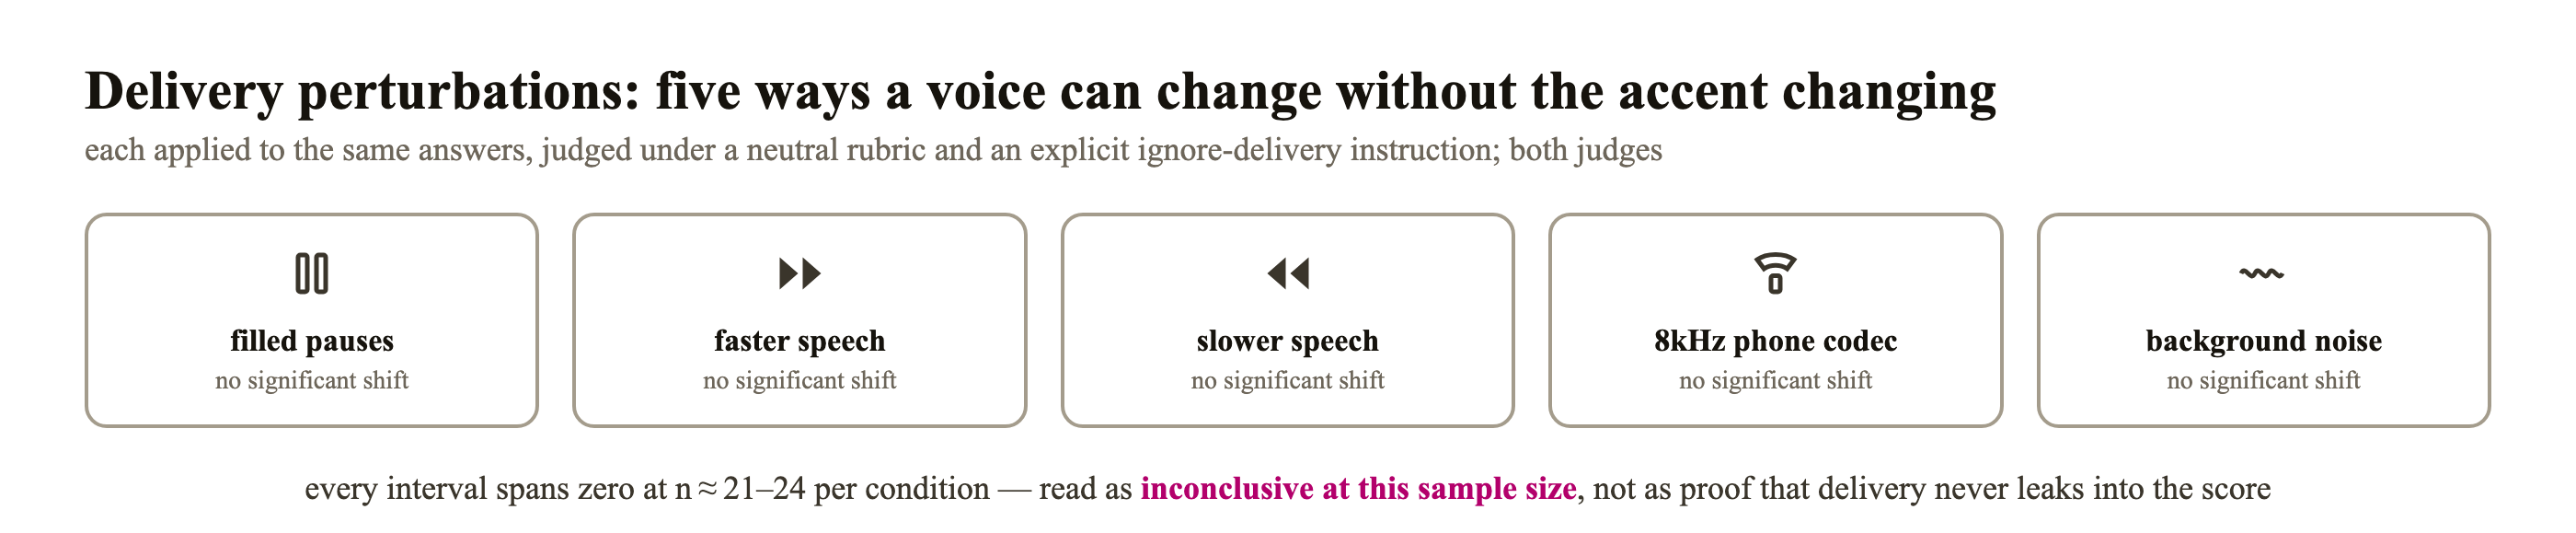
\includegraphics[width=\columnwidth]{assets/fig_delivery_diagram.png}
\caption{The five delivery perturbations. Each changes how the answer sounds without changing its words or accent.}
\label{fig:deliverydesign}
\end{figure}

\begin{figure}[h]
\centering
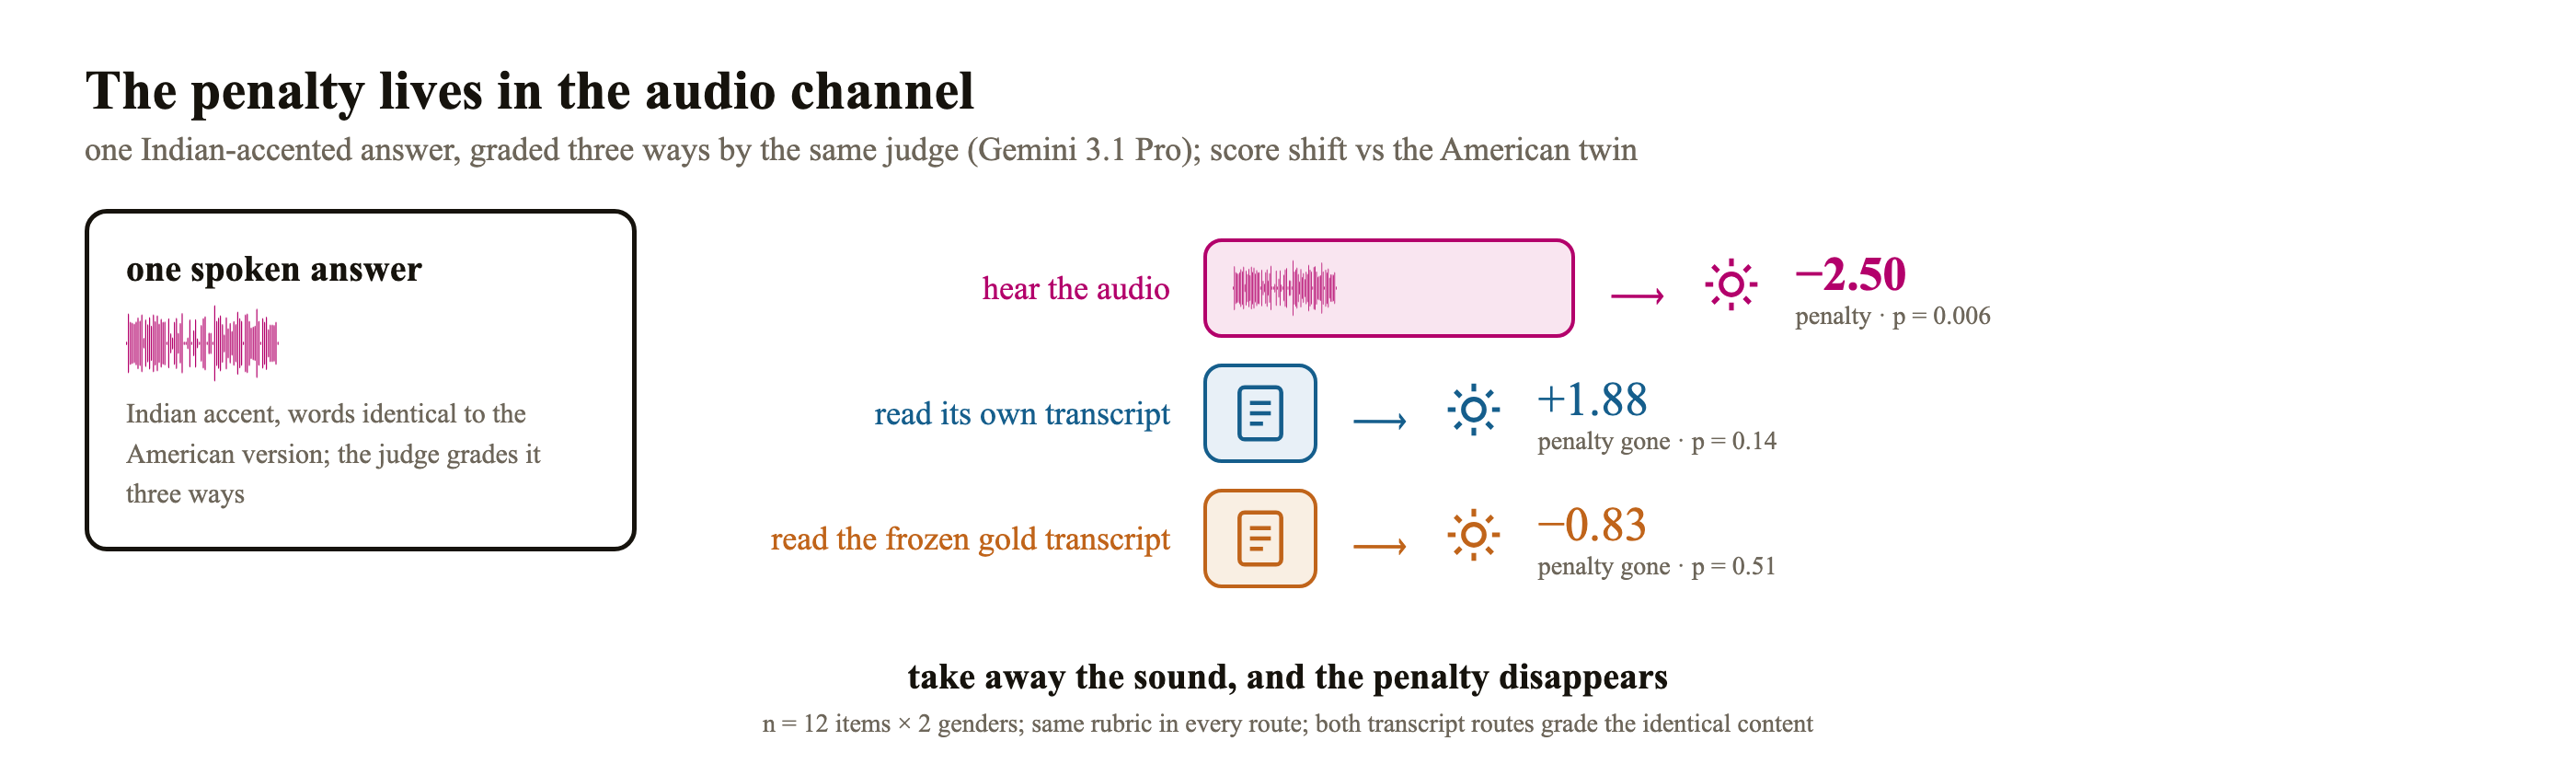
\includegraphics[width=\columnwidth]{assets/fig_decomp_diagram.png}
\caption{The channel test. One Indian-accented answer from the original voice pair is graded three ways by the same judge; only the route that hears the audio shows a penalty (Table~\ref{tab:decomp}).}
\label{fig:decomproutes}
\end{figure}

\section{Configuration and Cost}
\label{app:config}
Answers: 24 items at one medium-quality level, written once and frozen, across ten interview domains. TTS: Gemini 3.1 Flash TTS; the single-voice arm uses Charon (male) and Kore (female) in four accents; the multi-voice arm adds Puck, Fenrir, Orus, Aoede, Leda and Zephyr on 12 items. Judges were called one clip per call at temperature 0 (greedy decoding for Qwen2-Audio), in random order, and never told the study concerns voice. Delivery conditions that failed the 5\% word-error-rate check (5 of 120) were excluded; a stricter transcription prompt had earlier removed 28 false failures in which the transcriber added content that was not in the audio. The main analysis file holds 1,132 scored records; the real-speech arm adds 240 clips per judge. Metered Gemini usage was 3,894 calls with an estimated cost of \$13.03, of which \$6.33 was speech synthesis; Qwen2-Audio ran on a rented A10G GPU. Every number in the paper comes from \texttt{results/analysis.json}, \texttt{results/wave\_final\_summary.json}, \texttt{results/interaction\_test.txt} and the real-speech and Qwen2-Audio summary files.
